\documentclass[11pt,a4paper]{article}
\usepackage{fontspec}
\setmainfont{TeX Gyre Pagella}
\newfontfamily\headfont{Inter}[UprightFont=*-ExtraBold,BoldFont=*-ExtraBold,Extension=.otf,Path=/usr/share/fonts/opentype/inter/]
\usepackage[a4paper,margin=2.3cm]{geometry}
\usepackage{graphicx,booktabs,float,caption,array,xcolor}
\usepackage[hidelinks]{hyperref}
\usepackage{titlesec}
\usepackage[round]{natbib}
\usepackage{setspace}
\setstretch{1.05}
\renewcommand{\topfraction}{0.9}
\renewcommand{\bottomfraction}{0.8}
\renewcommand{\textfraction}{0.1}
\renewcommand{\floatpagefraction}{0.75}
\setlength{\parindent}{0pt}
\setlength{\parskip}{0.55em}
\titleformat{\section}{\headfont\Large}{\thesection}{0.8em}{}
\titleformat{\subsection}{\headfont\large}{\thesubsection}{0.8em}{}
\captionsetup{font=small,labelfont=bf}
\urlstyle{same}
\hypersetup{pdftitle={Dinner, Tea or Supper? What Britain Calls Its Evening Meal},pdfauthor={Tristan Hotham}}

\begin{document}
\begin{center}
{\Large\bfseries Dinner, Tea or Supper?\par}
\vspace{0.4em}
{\large What Britain calls its evening meal: mapping 12,522 answers\\from the Our Dialects survey\par}
\vspace{1.2em}
{\large Tristan Hotham\par}
\vspace{0.3em}
{\small Independent researcher\\
ORCID: 0000-0003-4931-9349\\
DOI: \href{https://doi.org/{{DOI}}}{https://doi.org/{{DOI}}}\par}
\vspace{0.8em}
2026
\end{center}

\begin{quote}
\small
\begin{center}\textbf{Abstract}\end{center}
The evening meal has three names in British English: dinner, tea and supper. I map 12,522 answers to the question ``what do you call your evening meal?'' from the Our Dialects survey (2013 to 2024), each placed at a postcode district with the respondent's age, gender and year of answer. Answers were smoothed with a Gaussian kernel whose width (16 km) was chosen by cross-validation, and the ``tea line'' was drawn where the smoothed shares of tea and dinner are equal. The divide is sharp: 75\% of answers from the north of England say tea and 74\% of answers from the south say dinner, with the Midlands split evenly. Wales leans to tea (57\%); Scotland (61\%) and Northern Ireland (79\%) to dinner. In logistic regressions, younger respondents in the south of England are more likely to say dinner (odds ratio 0.79 per decade of age, p $<$ 0.001), but there is no age gradient in the north (0.97, p = 0.22), and no rise in dinner across twelve survey years. Supper (3.6\%) is a word of older, southern respondents. Reweighted to regional populations, the survey reproduces YouGov's 2018 figures for England within a few points. The survey asks only about the evening meal, so the northern use of dinner for the midday meal is described from the literature rather than measured.

\textbf{Keywords:} dialect; British English; dialect geography; dinner; tea; supper; meal names; apparent time; Our Dialects; mapping
\end{quote}

\section{Introduction}
Few words divide Britain as cleanly as the name of the evening meal. In much of the north of England, the Midlands and Wales the cooked evening meal is tea, the main meal of the day is dinner and is eaten at midday, and supper is a snack before bed. In the south, the evening meal is dinner, the midday meal is lunch, and tea is a drink with a biscuit in the afternoon. The Oxford English Dictionary records the northern sense directly: tea is ``a light meal in the late afternoon, but locally in the U.K. (esp. northern) \ldots{} a cooked evening meal'' \citep{oed}. The choice is often read as a marker of class as well as region \citep{fox}.

This paper maps the evening meal from the largest public set of individual answers, the Our Dialects survey run from the University of Manchester \citep{ourdialects}, which has asked the question since 2013. \citet{mackenzie} have mapped tea against dinner from the same survey and set it beside the mid twentieth century Survey of English Dialects \citep{sed}. I add four things: a smoothed map with a cross-validated kernel and an explicit tea line; models of age, gender, survey year and region; the geography and age profile of supper; and a check against YouGov's 2018 poll of England \citep{yougov}. The work is a companion to a study of bread roll words from the same survey \citep{rolls}. An interactive version with a ``near you'' search is at \url{https://maps.tristanhotham.com/dinner-or-tea/}.

\section{Data}
\textbf{Survey answers.} The Our Dialects meal map was read from the project's public web map in 2026. It holds 12,555 answers, each with a point at the respondent's postcode district (slightly jittered), the postcode district itself, the year of answer (2013 to 2024), age, gender and the answer: dinner, tea or supper. The site's own legend reports the same total and shares (dinner 45.03\%, supper 3.56\%, tea 51.41\%). 33 answers from the Channel Islands and the Isle of Man were left out, leaving 12,522. The answers are \textcopyright{} the Our Dialects project and are not openly licensed: they are analysed here with credit and only aggregates with at least 10 answers are published.

\textbf{Who answered.} The survey is a volunteer online questionnaire. Its respondents are young (median age 22; 59\% under 25) and northern: 51\% of English answers come from the three northern regions, which hold 28\% of England's population, and 33\% from the North West alone (Table~\ref{tab:regions}). Women gave 7,363 answers and men 4,948.

\textbf{Geography and comparison figures.} Answers were placed in ONS regions and in counties (ceremonial counties in England, preserved counties in Wales, council areas in Scotland, Northern Ireland as one) using ONS boundaries \citep{ons_geo}. Regional populations are from the 2021 Census \citep{census}. YouGov's figures are quoted as published \citep{yougov}.

\begin{table}[tbp]\centering\small\caption{Answers by region. Sample and population columns: share of England's answers and of England's population (Census 2021), per cent.}\label{tab:regions}\begin{tabular}{lrrrrrr}\toprule Region & Answers & \% of sample & \% of pop. & Dinner \% & Tea \% & Supper \%\\\midrule
North East & 632 & 5.6 & 4.7 & 21.7 & 76.6 & 1.7\\
North West & 3,764 & 33.1 & 13.1 & 24.5 & 73.7 & 1.8\\
Yorkshire and The Humber & 1,421 & 12.5 & 9.7 & 21.0 & 77.2 & 1.8\\
East Midlands & 961 & 8.5 & 8.6 & 49.3 & 48.1 & 2.6\\
West Midlands & 917 & 8.1 & 10.5 & 46.9 & 50.3 & 2.8\\
East of England & 880 & 7.7 & 11.2 & 75.9 & 20.0 & 4.1\\
London & 870 & 7.7 & 15.6 & 86.8 & 6.7 & 6.6\\
South East & 1,201 & 10.6 & 16.4 & 74.8 & 18.2 & 7.0\\
South West & 718 & 6.3 & 10.1 & 57.0 & 34.7 & 8.4\\
Wales & 423 &  &  & 38.1 & 57.4 & 4.5\\
Scotland & 515 &  &  & 61.0 & 33.0 & 6.0\\
Northern Ireland & 220 &  &  & 78.6 & 19.5 & 1.8\\
\midrule All & 12,522 & & & 45.0 & 51.4 & 3.6\\\bottomrule\end{tabular}\end{table}

\section{Methods}
\textbf{Smoothing.} Answers were counted by word on a 2 km grid in British National Grid coordinates and smoothed with a Gaussian kernel, scaled so that each answer has weight one at its own spot. Each word's share is its smoothed count over the smoothed total, with a prior of one answer at the national shares. The kernel width was chosen by leave-one-cell-out prediction: each answer is predicted from the others with every answer in its own 2 km cell removed, and the mean log probability of the observed word is compared across widths of 4 to 32 km. It peaked at 16 km, although the curve is flat between 10 and 20 km. Where fewer than 10 kernel-weighted answers were nearby, the width was increased to 24 or 32 km; to avoid rings where the width changes, the step needed at each cell was spread with a 26 km maximum filter and a light Gaussian blur and the shares interpolated between neighbouring widths. Cells that still had fewer than 10 weighted answers were left blank, which leaves 86\% of UK land mapped. Halving or doubling the width leaves the leading word unchanged at 96\% and 96\% of answer locations.

\textbf{The tea line.} The tea line is the contour where the smoothed shares of tea and dinner are equal, kept where those are the two leading words; contours shorter than 12 km are dropped. The same rule gives short lines where supper overtakes.

\textbf{Models.} For dinner against tea (supper answers left out, n = 12,073) I fit logistic regressions of saying dinner on age (in decades, centred at 40), survey year (centred at 2018), gender (female, male, other or not given) and region, first for all answers and then separately for the north of England (North East, North West, Yorkshire and the Humber), the Midlands, the south (East of England, London, South East, South West), Scotland, Wales and Northern Ireland, with region effects inside each. A likelihood ratio test of an age by area interaction compares the slopes in the north, Midlands and south. A further model predicts supper against both other answers. Ages outside 10 to 90 were excluded (2 answers). Survey-year trends are also shown with each year's answers reweighted to the overall mix of region and six age groups. Models were fitted with statsmodels \citep{statsmodels}.

\textbf{Comparison with YouGov.} YouGov's 2018 figures are for adults in England. I took survey answers from people aged 18 and over in England and weighted each region's shares by its share of England's usual resident population in the 2021 Census.

\section{Results}
\subsection{The map and the tea line}
Figure~\ref{fig:map} shows the smoothed map. Tea leads across the north of England from the Scottish border to the Trent and across most of Wales; dinner leads across the south and east of England, the Scottish central belt and Northern Ireland. Of all answers, 75\% of the 5,817 from the north of England say tea and 74\% of the 3,669 from the south say dinner. The Midlands (1,878 answers) are split almost exactly: 49\% tea and 48\% dinner.

The tea line in England runs north from the Severn estuary past Gloucester and Worcester, swings round the west and north of Birmingham, then heads east past Derby and Nottingham, with Leicester on the dinner side, to the Wash. Along a north to south profile of England (Figure~\ref{fig:profile}) the smoothed share of tea rises from about a quarter across the southern counties to about three quarters north of the Mersey and the Humber, crossing one half in the band around Stoke, Derby and Nottingham. In Wales, 57\% of 423 answers say tea. In Scotland (515 answers) the map is broad brush: Glasgow and the west are firmly dinner (smoothed 83\%), while Edinburgh, Fife and the north-east are closer to even or lean to tea. Northern Ireland (220 answers) is 79\% dinner. Across the UK, 58\% of answers come from places on the tea side of the line.

\begin{figure}[tbp]\centering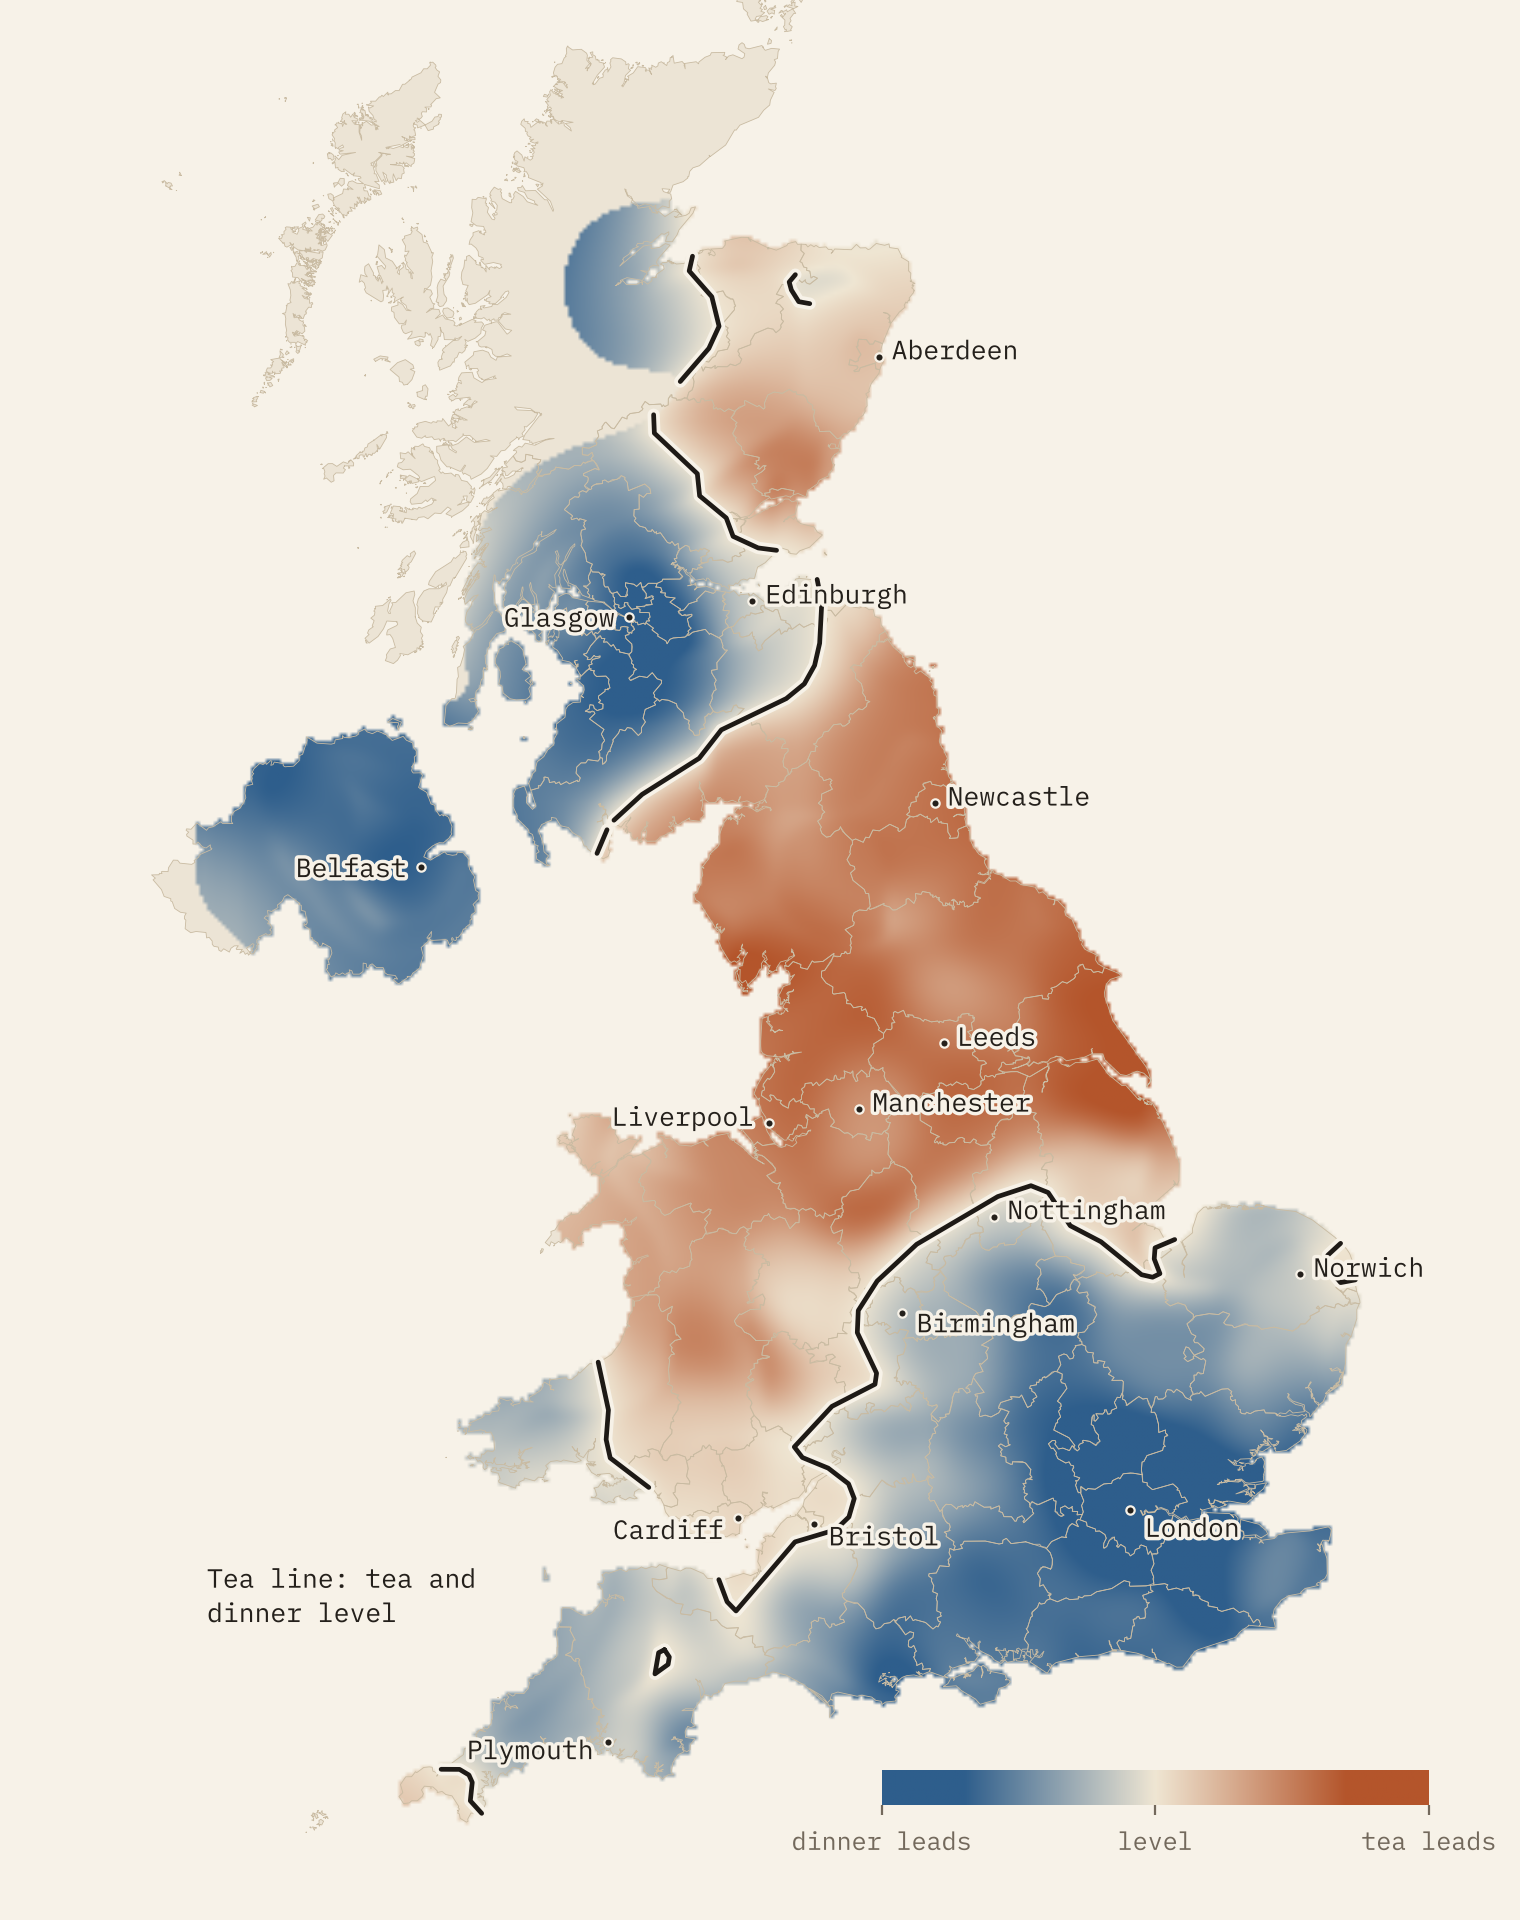
\includegraphics[width=.78\textwidth]{f_map.png}
\caption{Tea against dinner, smoothed. Brown: tea leads; blue: dinner leads; paler colours mark a closer split. The black line is the tea line, where the smoothed shares are equal. Blank areas have fewer than 10 weighted answers nearby.}\label{fig:map}\end{figure}

\begin{figure}[tbp]\centering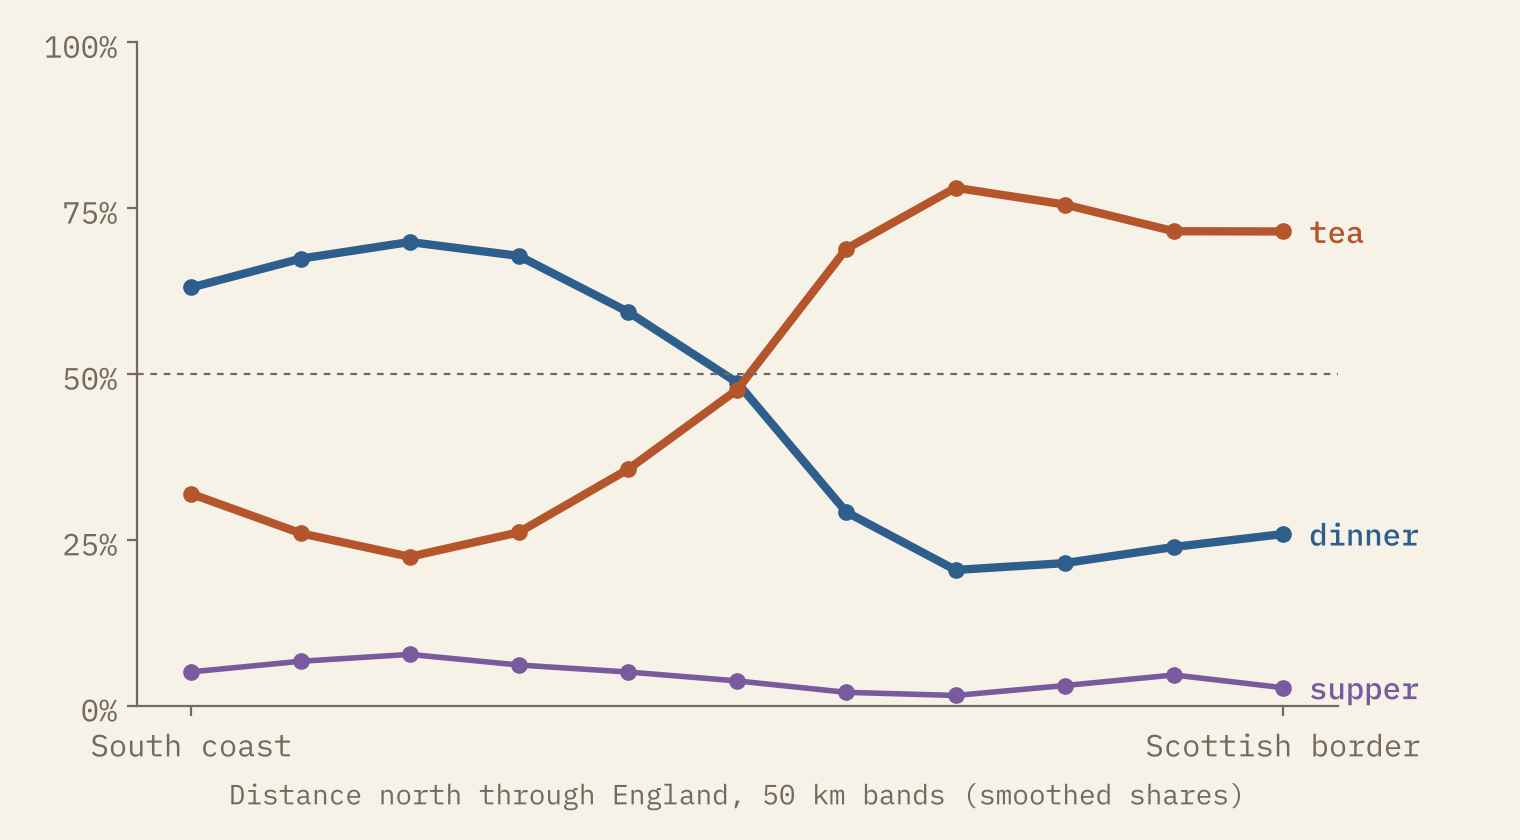
\includegraphics[width=.86\textwidth]{f_profile.png}
\caption{Mean smoothed share of each word in 50 km bands of northing across England (bands with at least 50 answers).}\label{fig:profile}\end{figure}

\subsection{Regions and counties}
Every northern English region has a tea majority above 70 per cent and every southern region a dinner majority (Figure~\ref{fig:regions}). Among the 57 counties with at least 30 answers, tea leads in 24 and dinner in 33. The most tea counties are the East Riding of Yorkshire (81\%) and Lancashire (80\% of 846); the least are Greater London (7\% tea, 87\% dinner) and Hertfordshire. The Our Dialects site text gives London as 89\% dinner and 3\% tea, apparently from an earlier count.

\begin{figure}[tbp]\centering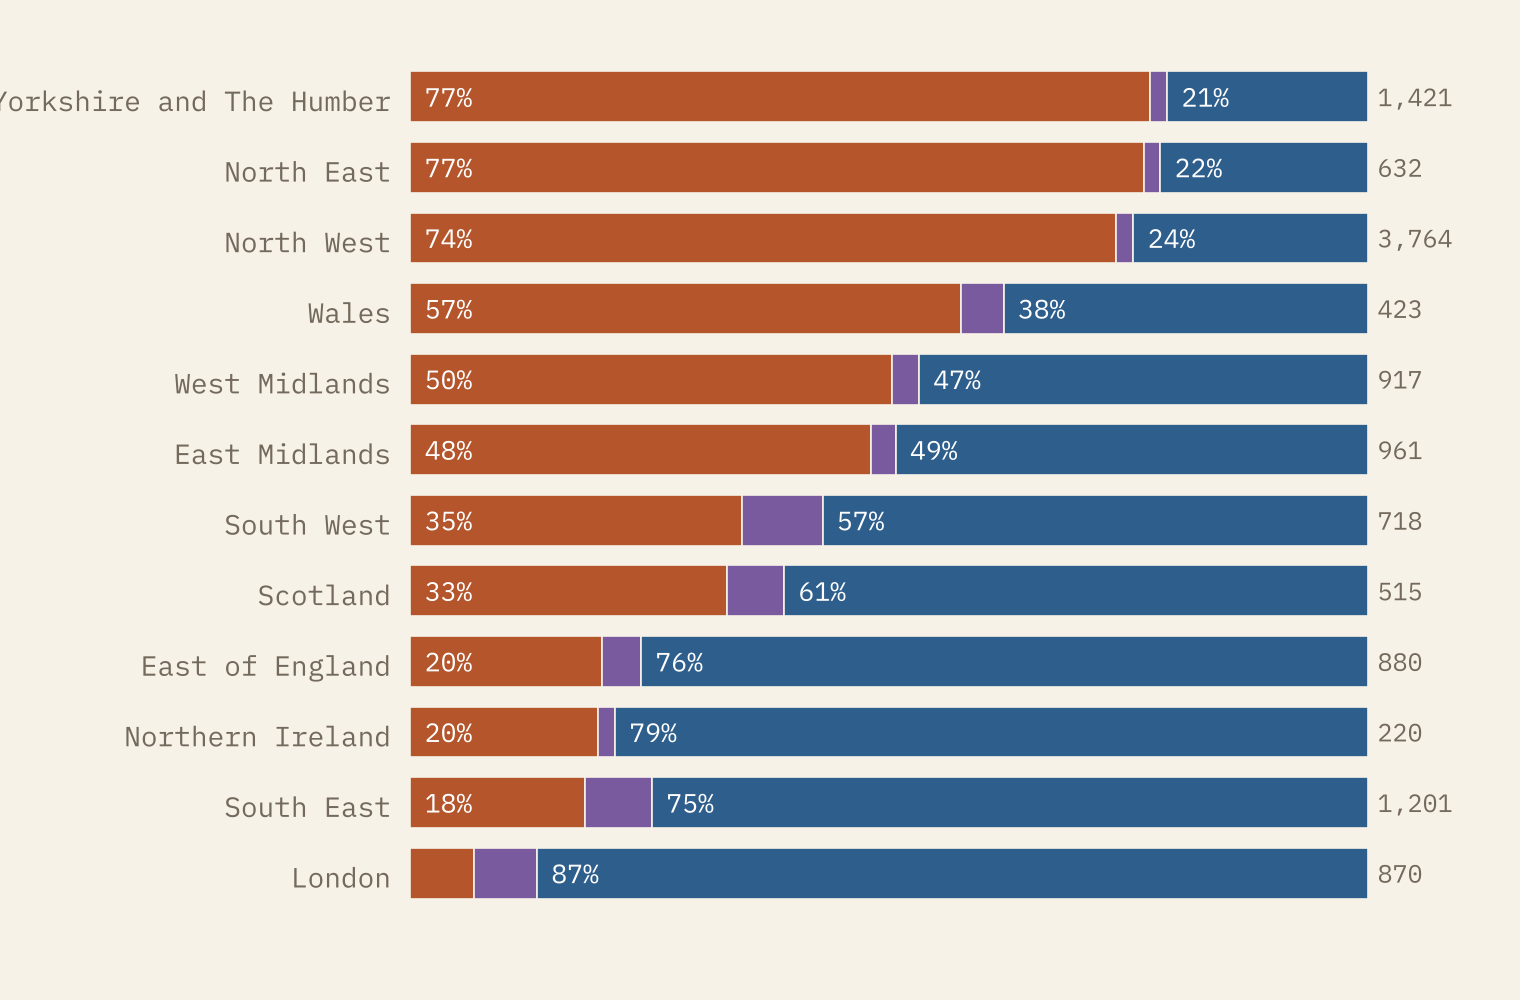
\includegraphics[width=.86\textwidth]{f_regions.png}
\caption{Share of answers giving each word, by region (tea, supper, dinner from left), with numbers of answers.}\label{fig:regions}\end{figure}

\subsection{Age, survey year and gender}
Region dominates. A model with region alone has a McFadden pseudo R\textsuperscript{2} of 0.195, against 0.200 with age, year and gender added and 0.007 for age, year and gender without region (Table~\ref{tab:model}). Relative to the North West, the odds of dinner are 40 times higher in London and 13 times higher in the South East.

Age matters only in some places (Figure~\ref{fig:age}, Table~\ref{tab:age}). In the south of England, 79\% of answers from people aged 18 to 24 say dinner against 57\% from those aged 50 to 64; the odds of dinner fall by a factor of 0.79 per decade of age (95\% interval 0.74 to 0.84, p $<$ 0.001). The slope is weaker in the Midlands (0.91, p = 0.005) and in Scotland (0.81, p = 0.001), and absent in the north of England (0.97, 95\% interval 0.93 to 1.02, p = 0.22), Wales and Northern Ireland. The slopes in the north and south differ (likelihood ratio 31.4 on 2 degrees of freedom, p $<$ 0.001). From the southern model, the predicted share saying dinner is 83\% at age 20 and 66\% at age 60; in the north it is 24\% and 22\%.

Read in apparent time, this suggests that dinner is still spreading in the south and Midlands, where it is already the majority word, but not making inroads into the north. Two other readings fit equally well: people may change words over the life course, and age is entangled with other things the survey does not record, such as class and whether people have moved. Real time gives no support to a spread. Reweighted to the same mix of region and age, dinner's share by survey year ranges between 41\% and 50\% with no upward trend (Figure~\ref{fig:year}), and in the full model the odds of dinner fall slightly with survey year (0.969 per year, p $<$ 0.001). Twelve years is a short window, and the kinds of people answering changed over the period (the median age of respondents rose from 21 to 28), so this is weak evidence either way.

Gender makes no difference: 52\% of women and 52\% of men say tea (chi-squared p = 0.80; in the model the odds ratio for men is 0.95, p = 0.22). Respondents who gave another gender or none said dinner more often (1.51, p = 0.02), on 211 answers.

\begin{table}[tbp]\centering\small\caption{Logistic regression of saying dinner rather than tea (n = 12,073). Odds ratios with 95\% intervals; regions against the North West. McFadden pseudo R\textsuperscript{2} 0.200.}\label{tab:model}\begin{tabular}{lrrr}\toprule Term & Odds ratio & 95\% interval & p\\\midrule
Age (per decade) & 0.90 & 0.88 to 0.93 & $<$ 0.001\\
Survey year (per year) & 0.97 & 0.96 to 0.98 & $<$ 0.001\\
Male (against female) & 0.95 & 0.87 to 1.03 & 0.22\\
Other or not given & 1.51 & 1.08 to 2.12 & 0.02\\
\midrule
North East & 0.90 & 0.74 to 1.11 & 0.34\\
Yorkshire and The Humber & 0.84 & 0.73 to 0.98 & 0.03\\
East Midlands & 3.27 & 2.81 to 3.80 & $<$ 0.001\\
West Midlands & 2.88 & 2.47 to 3.36 & $<$ 0.001\\
East of England & 11.85 & 9.85 to 14.25 & $<$ 0.001\\
London & 40.09 & 30.35 to 52.95 & $<$ 0.001\\
South East & 12.96 & 10.95 to 15.33 & $<$ 0.001\\
South West & 5.22 & 4.38 to 6.24 & $<$ 0.001\\
Wales & 2.06 & 1.66 to 2.56 & $<$ 0.001\\
Scotland & 6.39 & 5.19 to 7.85 & $<$ 0.001\\
Northern Ireland & 12.40 & 8.80 to 17.49 & $<$ 0.001\\
\bottomrule\end{tabular}\end{table}

\begin{figure}[tbp]\centering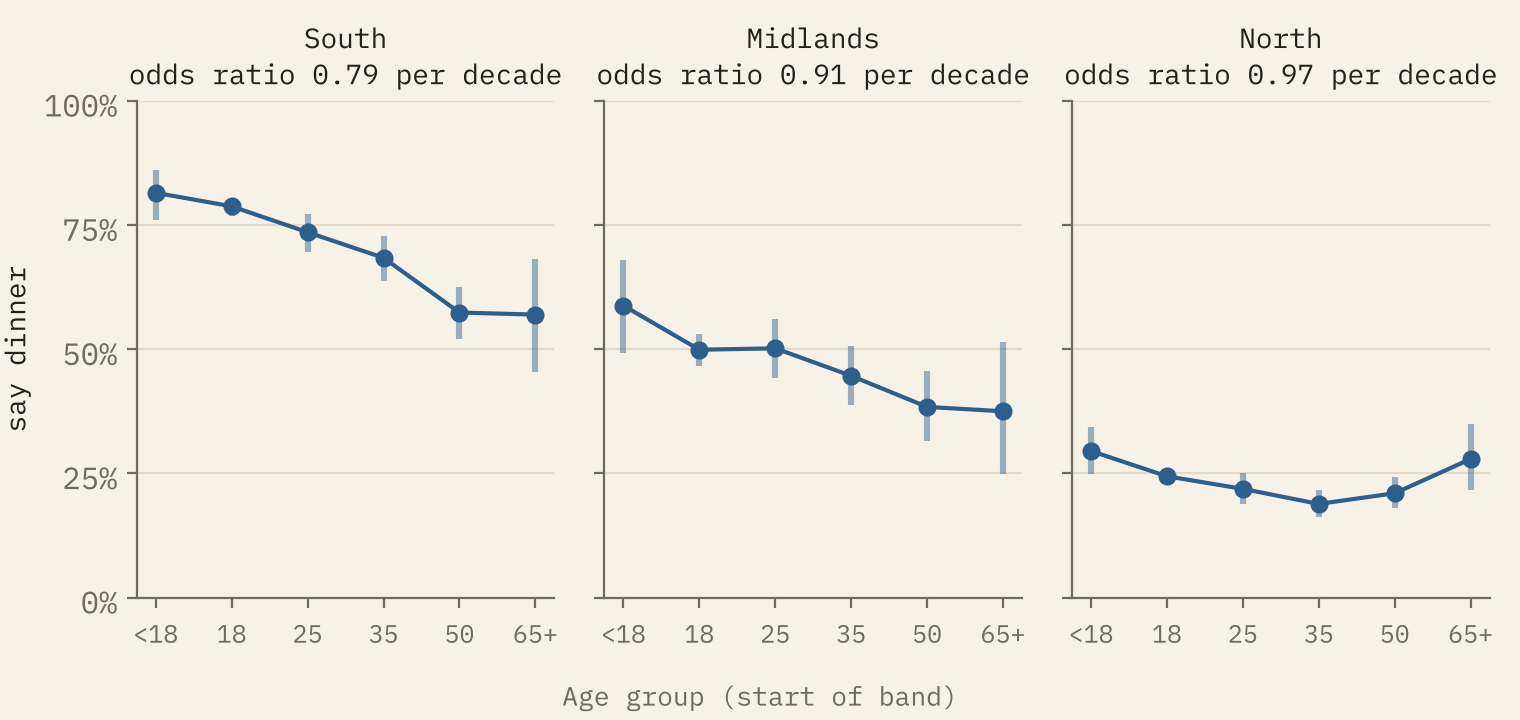
\includegraphics[width=.92\textwidth]{f_age.png}
\caption{Share saying dinner by age group, with 95\% exact binomial intervals, in the south, Midlands and north of England. Odds ratios per decade from separate logistic regressions with region, year and gender.}\label{fig:age}\end{figure}

\begin{table}[tbp]\centering\small\caption{Age slope for dinner against tea, fitted separately in each area (with survey year, gender and, where there is more than one, region). Odds ratio per decade of age; below 1, younger people say dinner more.}\label{tab:age}\begin{tabular}{lrrrr}\toprule Area & Answers & Odds ratio & 95\% interval & p\\\midrule
North & 5,712 & 0.97 & 0.93 to 1.02 & 0.22\\
Midlands & 1,826 & 0.91 & 0.85 to 0.97 & 0.005\\
South & 3,431 & 0.79 & 0.74 to 0.84 & $<$ 0.001\\
Scotland & 484 & 0.81 & 0.71 to 0.92 & 0.001\\
Wales & 404 & 0.94 & 0.81 to 1.10 & 0.47\\
Northern Ireland & 216 & 0.87 & 0.68 to 1.12 & 0.29\\
\bottomrule\end{tabular}\end{table}

\begin{figure}[tbp]\centering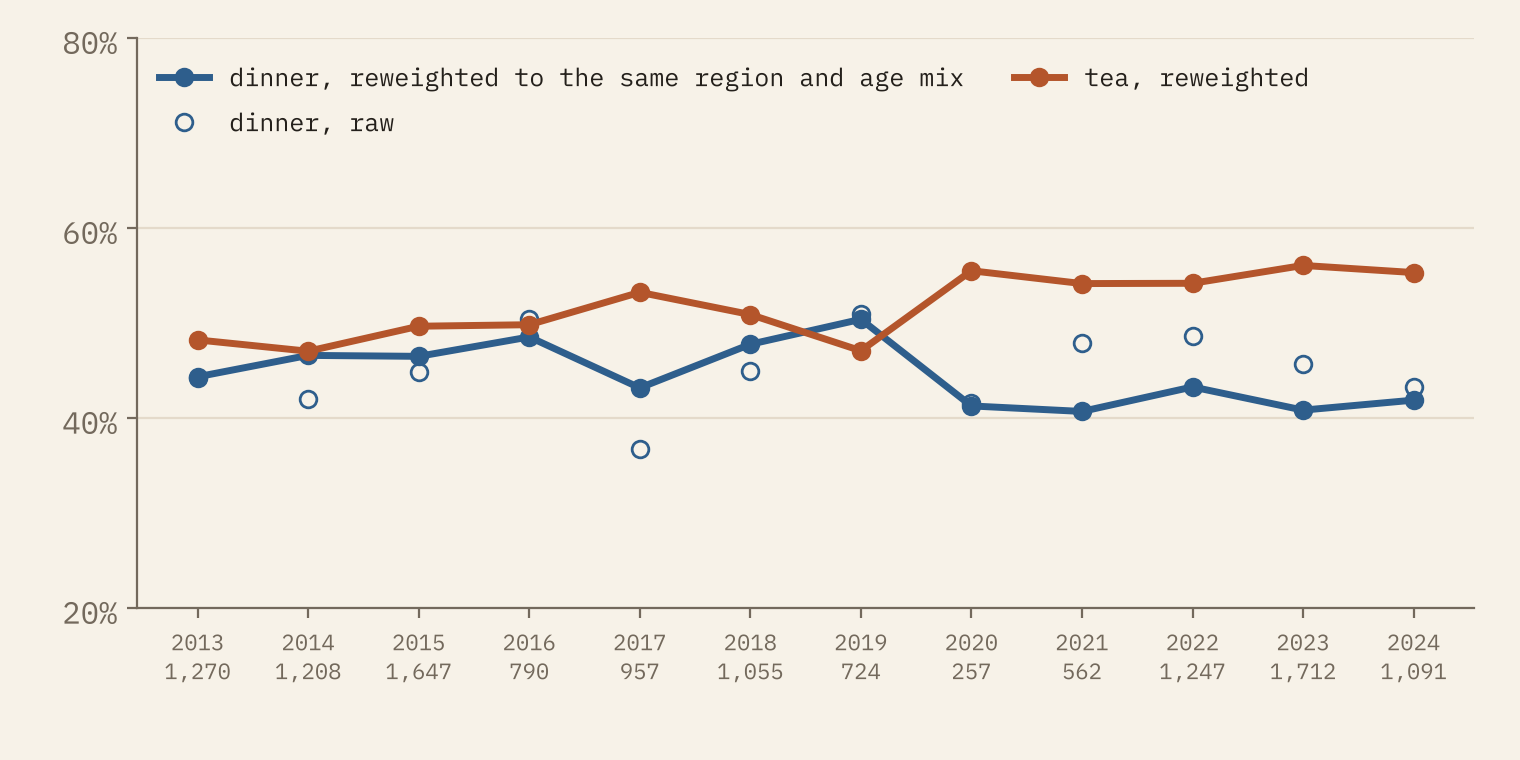
\includegraphics[width=.86\textwidth]{f_year.png}
\caption{Share saying dinner and tea by survey year, raw and reweighted to the overall mix of region and age group. Answers per year below each year.}\label{fig:year}\end{figure}

\subsection{Supper}
Supper is given in 447 answers (3.6\%). It is most common in the South West (8.4\%), the South East (7.0\%), London (6.6\%) and Scotland (6.0\%), and least common in the north of England and Northern Ireland (under 2\%). It rises steeply with age (Figure~\ref{fig:supper}): among southern respondents aged 65 and over 20\% say supper, against 6\% at 18 to 24, and across the UK the odds of supper rise by 1.34 per decade (p $<$ 0.001). Supper leads the smoothed map only in a small area of Aberdeenshire, where 11 of 32 answers say it.

\begin{figure}[tbp]\centering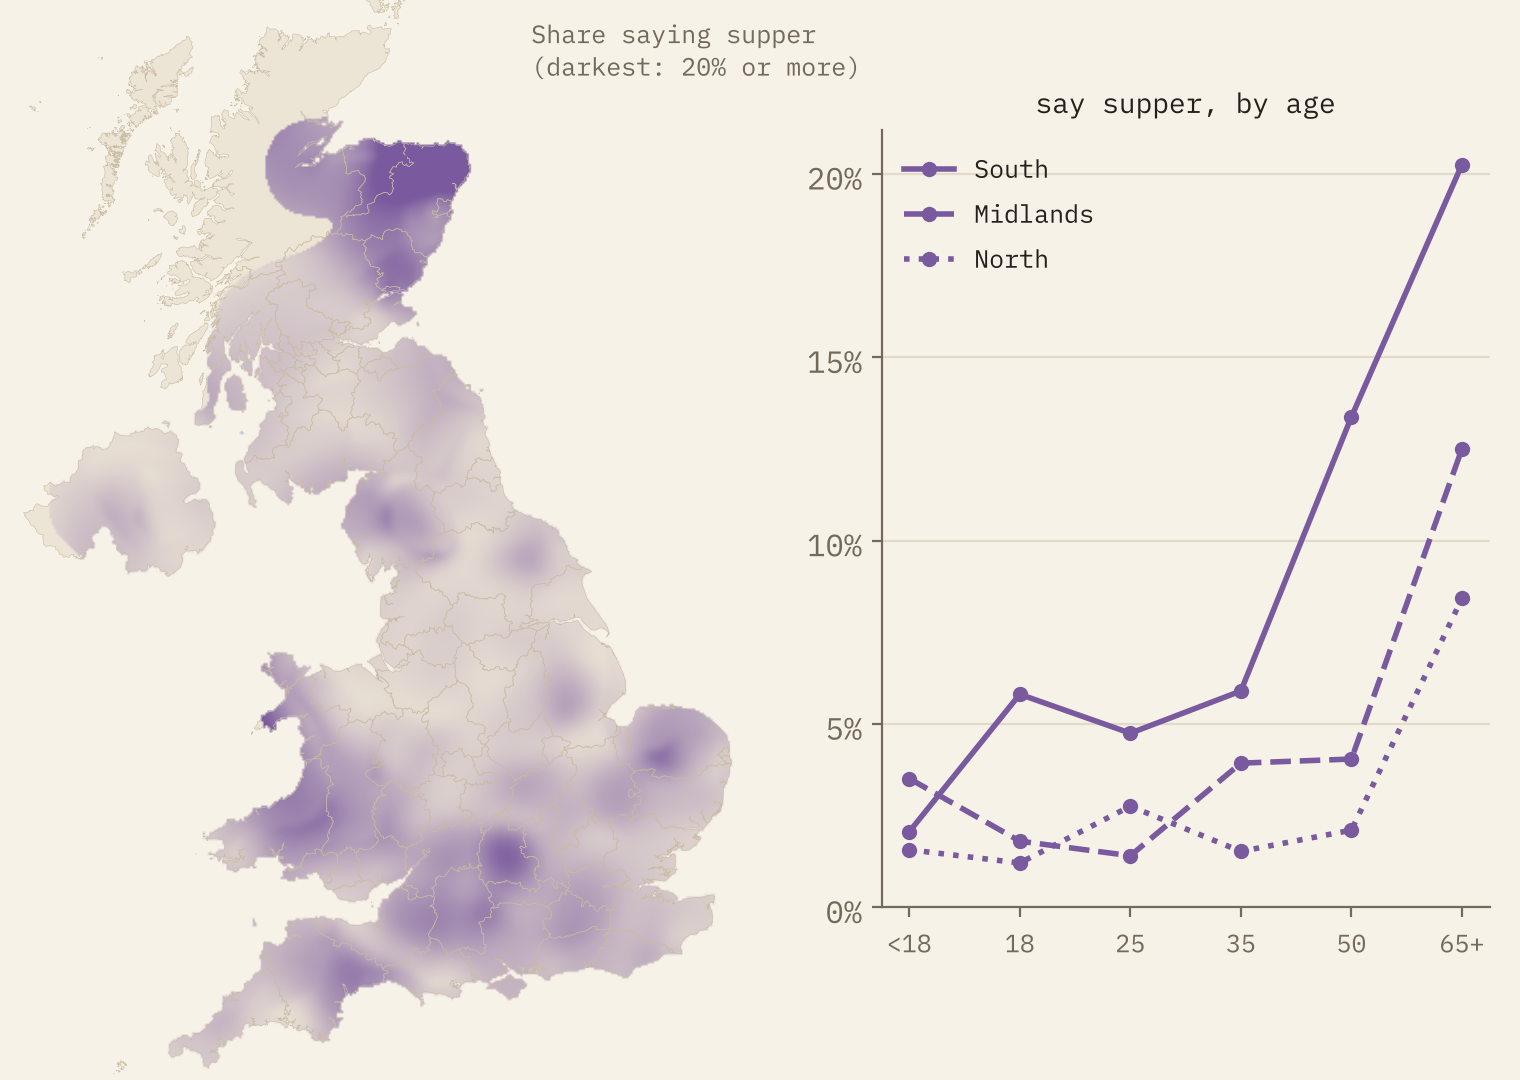
\includegraphics[width=.92\textwidth]{f_supper.png}
\caption{Left: smoothed share saying supper (dashed lines: where supper overtakes). Right: share saying supper by age group.}\label{fig:supper}\end{figure}

\subsection{Comparison with YouGov}
YouGov's 2018 survey of more than 42,000 adults in England found 57\% dinner, 36\% tea and 5\% supper \citep{yougov}. The raw survey answers from England (44\% dinner, 53\% tea) are far from this because of who answered. Weighted to regional populations, the adult answers give 55.0\% dinner, 40.3\% tea and 4.6\% supper, within five points of YouGov on every word (Figure~\ref{fig:yougov}). YouGov's three most dinner counties (East Sussex, Essex, Kent) rank 4th, 3rd and 7th for dinner of the 45 English counties here with at least 30 answers, and its three most tea counties (Greater Manchester, Tyne and Wear, Merseyside) rank 12th, 3rd and 6th for tea. YouGov also reported social grade: in the north 58\% of middle-class and 67\% of working-class respondents said tea; in the south 74\% and 70\% said dinner. The Our Dialects survey records no class measure.

\begin{figure}[tbp]\centering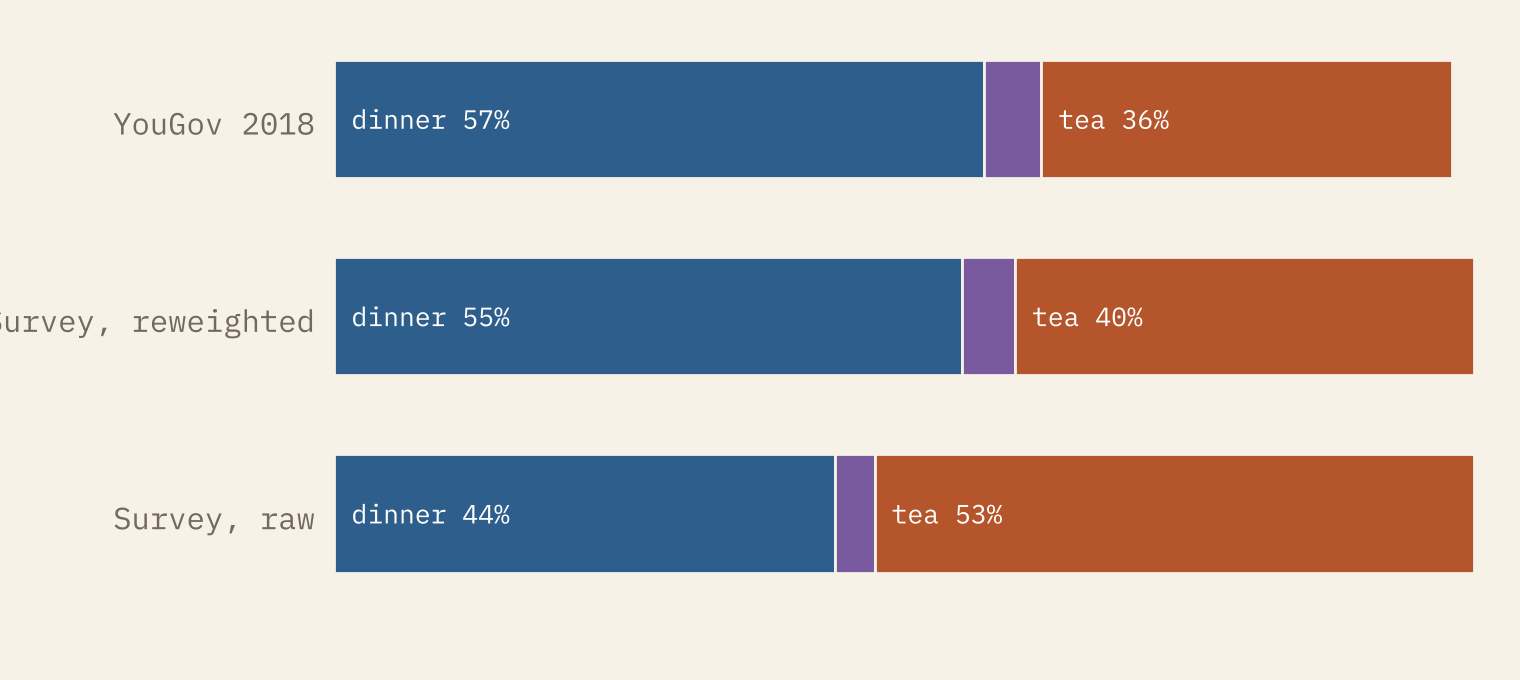
\includegraphics[width=.86\textwidth]{f_yougov.png}
\caption{England: YouGov 2018 against the survey, raw and with adult answers reweighted to regional populations (2021 Census).}\label{fig:yougov}\end{figure}

\section{Discussion}
The tea line is one of the clearest boundaries in British dialect geography, and it crosses England close to where the better known north and south divides in vowels run, from the Severn to the Wash. The age pattern suggests that the boundary is stable in the north and that the south is consolidating rather than advancing: younger southerners are more consistently ``dinner'', but younger northerners are as ``tea'' as their parents. That fits a picture in which tea is not a fading rural word but the ordinary word of the industrial north, tied to the working day and to the midday dinner of school and work. It also fits the class reading: a southern, middle-class dinner has not displaced northern tea in twenty-first century answers.

The survey cannot see the other half of the system. Where tea is the evening meal, dinner is usually the midday meal, and supper a late snack; the survey asks only about the evening. In the Ribble Valley in Lancashire, for example, 73\% of 55 answers say tea, and local usage of dinner for the midday meal is well attested, but nothing here measures it.

\section{Limitations}
The survey is a volunteer sample, heavily northern and young; maps are sharpest where it was popular and blank where it was not. Each person chose one of three words for the evening meal, which flattens people who use more than one, and there is no question about the midday meal. Answers are placed at postcode districts and may record where people live rather than where they grew up. Age differences in a single survey are consistent with change in progress but also with life-course change and with unmeasured class and mobility. Scotland, Wales and Northern Ireland have few answers. The YouGov comparison uses only region for weighting, not age, sex or class. All counts are for the answers on the public map in 2026.

\section{Conclusion}
Tea is the evening meal across the north of England and most of Wales; dinner across the south, the Scottish central belt and Northern Ireland; and the line between them runs across the Midlands from the Severn to the Wash. Younger southerners say dinner more consistently than older ones, but there is no sign of dinner moving north, and none of it rising across twelve years of answers. Supper is the word of older people in the south.

\section*{Data and code availability}
The interactive map is at \url{https://maps.tristanhotham.com/dinner-or-tea/}. Code and aggregate data (hexagons, counties, regions and postcode areas with at least 10 answers, the tea line, and results) are at \url{https://github.com/Tristan-Hotham/dinner-or-tea} and archived with this paper at \url{https://doi.org/{{DOI}}}. The individual survey answers are not redistributed; they belong to the Our Dialects project. Derived data and text are released under CC BY 4.0, code under the MIT licence.

\section*{AI statement}
I wrote the text, with drafting and editing assistance from Claude (Anthropic), which also helped prepare the analysis code. I reviewed and checked all text and results.

\begin{thebibliography}{9}
\bibitem[Fox(2004)]{fox} Fox, K. (2004) \emph{Watching the English: The Hidden Rules of English Behaviour}. London: Hodder and Stoughton.
\bibitem[Hotham(2026)]{rolls} Hotham, T. (2026) Barm, bap, cob or roll? Mapping Britain's bread roll lines from 20,000 survey answers. Zenodo. \url{https://doi.org/10.5281/zenodo.23691943}
\bibitem[MacKenzie et al.(2022)]{mackenzie} MacKenzie, L., Bailey, G. and Turton, D. (2022) Towards an updated dialect atlas of British English. \emph{Journal of Linguistic Geography}. Lancaster University eprint 168083, \url{https://eprints.lancs.ac.uk/id/eprint/168083/}
\bibitem[Office for National Statistics(2022)]{census} Office for National Statistics (2022) Census 2021: population and household estimates, England and Wales. Open Government Licence v3.0.
\bibitem[Office for National Statistics(2023)]{ons_geo} Office for National Statistics (2023) Regions, counties and local authority boundaries. Open Government Licence v3.0. Contains OS data \textcopyright{} Crown copyright and database right.
\bibitem[Orton and Dieth(1962)]{sed} Orton, H. and Dieth, E. (eds) (1962 to 1971) \emph{Survey of English Dialects}. Leeds: E. J. Arnold.
\bibitem[Our Dialects(2026)]{ourdialects} Our Dialects (2026) What do you call your evening meal? Our Dialects map, University of Manchester. \url{https://www.ourdialects.uk/maps/meal/}
\bibitem[Oxford English Dictionary(2013)]{oed} Oxford English Dictionary (2013) tea, n. Oxford University Press.
\bibitem[Seabold and Perktold(2010)]{statsmodels} Seabold, S. and Perktold, J. (2010) statsmodels: econometric and statistical modeling with Python. \emph{Proceedings of the 9th Python in Science Conference}.
\bibitem[YouGov(2018)]{yougov} YouGov (2018) Dinner time or tea time? It depends where you live. \url{https://yougov.com/en-gb/articles/20826-dinner-time-or-tea-time-it-depends-where-you-live}
\end{thebibliography}
\end{document}
